\hspace{3mm}

\centerline{\bf \Huge Домашнее задание. Теория игр.}

\begin{flushright}
    \scriptsize{Ты думаешь, что ты понял это, \\хотя на самом деле всего лишь думаешь,\\ что ты понял то, о чем ты думаешь. \\Хатаке Какаши. Наруто}
\end{flushright}


\problem{1!} Внутрь прямоугольника размерами $10\times100$ Герман и Алина по очереди кладут палочки длины 10. Палочки должны находиться строго внутри прямоугольника и не пересекаться с другими. Считается, что у палочек есть какая-то маленькая толщина. Проигрывает тот, кто не сможет сделать ход. Алина начинает первая.

\problem{2!} Герман и Дольган попали в гендзюцу Ердема под названием шахматное цукуёми. В ряд выложены 2002 пешки, пронумерованные от 1 до 2002. За один ход каждый из них может менять местами две пешки находящиеся через одну друг от друга. Смогут ли они договориться так, чтобы спустя несколько ходов расположить пешки в обратном порядке или они навсегда застряли в гендзюцу Ердема?

\problem{3} В кастрюле лежит 2027 беригов. Герман и Ердем по очереди съедают из кастрюли от 1 до 17 беригов. Когда кастрюля опустошается, игроки подсчитывают съеденное количество беригов. Если эти числа взаимно просты – выигрывает Ердем, в противном случае выигрывает Герман. Ердем ходит первым.

\problem{4} Герман и Анджур Аркадьевич играют в следующую игру. Герман выписывает подряд цифры 0 или 1 в произвольном порядке, пока не получится 2023-значное число. Каждый раз, когда Герман выставляет цифры, Анджур Аркадьевич меняет местами две уже написанные цифры(первый ход он пропускает, а остальные обязательно ходит!) Если итоговое число получится палиндромом(то есть будет читаться с обеих сторон одинаково), то Анджур Аркадьевич побеждает, если нет, то побеждает Герман.

%https://problems.ru/view_problem_details_new.php?id=98434

\problem{5}\textbf{Бонусная задача!} Дана таблица $m\times n$, заполненная целыми числами. За ход Герману разрешается поменять местами две строчки, умножить все числа строчки на $-1$ или же отнять от одной строчку другую, умноженную на некоторое целое число. Сможет ли он с помощью этих операций добиться вот такой таблицы? Здесь числа $m_1, m_2, \dotsc, m_r$ натуральные, причем каждое следующее делится на предыдущее.

\begin{figure}[h] 
    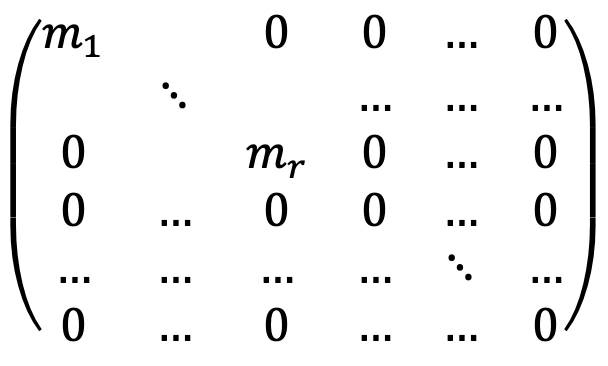
\includegraphics[scale=0.5]{V блок/Киви/lessons_5-6/matrix.png}
\end{figure}